\documentclass{article}
\usepackage[utf8]{inputenc}
\usepackage[T1]{fontenc}
\usepackage{lmodern} % Important for scalable fonts
\usepackage[english]{babel}
\usepackage{amsmath,amssymb,physics,graphicx,xcolor,amsthm}
\usepackage[expansion=false]{microtype} % Microtype with disabled expansion
\usepackage{hyperref}
\usepackage{booktabs}
\usepackage{siunitx}
\usepackage{cleveref}
\usepackage{pgfplots}
\pgfplotsset{compat=1.18}
\usepackage{tikz}
\usetikzlibrary{intersections}
\usepgfplotslibrary{fillbetween}
\bibliographystyle{plain} % or another style
\usepgfplotslibrary{fillbetween}
% Font settings
\renewcommand{\familydefault}{\rmdefault} % Serif font as standard

% Hyperref setup
\hypersetup{
	colorlinks=true,
	linkcolor=blue,
	urlcolor=blue,
	citecolor=red,
	pdftitle={From Time Dilation to Mass Variation},
	pdfauthor={Johann Pascher},
	pdfsubject={Theoretical Physics},
	pdfkeywords={Time-Mass Duality, Lagrangian Density, Quantum Field Theory}
}

% Theorem styles
\newtheorem{theorem}{Theorem}[section]
\newtheorem{proposition}[theorem]{Proposition}
\newtheorem{corollary}[theorem]{Corollary}
\newtheorem{lemma}[theorem]{Lemma}

\theoremstyle{definition}
\newtheorem{definition}[theorem]{Definition}
\newtheorem{example}[theorem]{Example}

\theoremstyle{remark}
\newtheorem{remark}[theorem]{Remark}
\newcommand{\HiggsLagr}{\mathcal{L}_{\text{Higgs-T}}}
\newcommand{\DhiggsT}{\mathcal{D}_\mu\Phi_T}
\renewcommand{\proofname}{Proof}

% Custom commands
\newcommand{\Tfield}{T(x)} % Intrinsic time as a field
\newcommand{\DcovT}[1]{\Tfield D_\mu #1 + #1 \partial_\mu \Tfield}
\newcommand{\DhiggsTdef}{\Tfield (\partial_\mu + igA_\mu)\Phi + \Phi \partial_\mu \Tfield}
\usepackage{mathtools} % For better error messages


% For long equations
\allowdisplaybreaks
\emergencystretch=1em

\title{From Time Dilation to Mass Variation: A Complete Reformulation of the Lagrangian Density}
\author{Johann Pascher}
\date{March 30, 2025}

\begin{document}
	
	\maketitle
	
	\begin{abstract}
		This work presents a detailed derivation and mathematical formulation of the Lagrangian density within the framework of time-mass duality theory. Starting from the basic principles of this theory - the duality between a standard picture with time dilation and constant rest mass and an alternative picture with absolute time and variable mass - a consistent field theory is developed. The central innovation is the introduction of intrinsic time $T = \hbar/mc^2$ as a fundamental quantity that is directly connected to mass and determines the temporal evolution of all quantum systems. The resulting Lagrangian density includes modified terms for the Higgs field, fermions, gauge bosons, and their interactions, with the Higgs field playing a special role as a mediator between the two complementary descriptions. The work shows that this reformulation is not only mathematically consistent but also leads to experimentally verifiable predictions that deviate from the Standard Model of particle physics.
	\end{abstract}
	
	\tableofcontents
	\newpage
	
	\section{Introduction}
	
	The time-mass duality theory represents an innovative approach that reconsiders central concepts of modern physics in a new light. In contrast to the conventional view, where time is considered relative (time dilation) and rest mass as constant, this theory postulates an alternative, mathematically equivalent picture where time remains absolute and instead the mass varies. This duality requires a fundamental reformulation of established physical theories, particularly the Lagrangian density that describes the dynamics of all fundamental fields and their interactions.
	
	\subsection{Basic Principles of Time-Mass Duality}
	
	The time-mass duality theory is based on the following fundamental principles:
	
	\begin{itemize}
		\item \textbf{Intrinsic Time:} For every particle with mass $m$, a characteristic intrinsic time is defined as $T = \frac{\hbar}{mc^2}$. This time scales inversely with mass and determines the temporal evolution of the quantum system.
		
		\item \textbf{Field-Theoretical Extension:} The intrinsic time is treated as a dynamic field $\Tfield$ that can depend on space and time and is coupled to the Higgs field and thus to mass generation.
		
		\item \textbf{Modified Time Derivative:} The conventional time derivative $\frac{\partial}{\partial t}$ is replaced by a modified time derivative that considers the intrinsic time scale of the system and can be space- and time-dependent.
		
		\item \textbf{Duality of Descriptions:} There exist two equivalent descriptions of physical phenomena:
		\begin{enumerate}
			\item The \textbf{standard picture} with time dilation ($t' = \gamma t$) and constant rest mass ($m_0 = \text{const.}$)
			\item The \textbf{alternative picture} with absolute time ($T_0 = \text{const.}$) and variable mass ($m = \gamma m_0$)
		\end{enumerate}
		
		\item \textbf{Higgs Mediation:} The Higgs field plays a central role as a mediator between both descriptions by defining both the rest mass and the intrinsic time scale.
	\end{itemize}
	
	\subsection{Goal and Structure of This Work}
	
	The main goal of this work is the development of a complete and consistent mathematical formulation of the Lagrangian density within the framework of time-mass duality theory. This formulation must encompass all fundamental interactions and fields of the Standard Model while correctly reflecting the novel aspects of duality theory.
	
	The work is structured as follows:
	
	\begin{itemize}
		\item Section 2 mathematically derives intrinsic time and discusses its physical significance.
		\item Section 3 addresses the transformation of fundamental field equations according to the principle of time-mass duality.
		\item Section 4 develops the modified Lagrangian density for scalar fields, particularly the Higgs field.
		\item Section 5 reformulates the Lagrangian density for fermions and their coupling to the Higgs field.
		\item Section 6 treats the modified Lagrangian density for gauge bosons.
		\item Section 7 presents the complete total Lagrangian density and verifies its consistency.
		\item Section 8 examines the experimental consequences and predictions of this theory.
		\item Section 9 summarizes the results and provides an outlook for further research.
	\end{itemize}
	
	\section{Mathematical Derivation of Intrinsic Time}
	
	\subsection{Basic Concepts and Definitions}
	
	To establish intrinsic time as a fundamental quantity, we begin with the basic relationships from special relativity and quantum mechanics.
	
	\begin{definition}[Energy-Mass Equivalence]
		Special relativity postulates the equivalence of mass and energy according to the famous formula
		\begin{equation}
			E = mc^2
		\end{equation}
		where $E$ is energy, $m$ is mass, and $c$ is the speed of light in vacuum.
	\end{definition}
	
	\begin{definition}[Energy-Frequency Relationship]
		Quantum mechanics connects the energy of a quantum mechanical system with its frequency through
		\begin{equation}
			E = h\nu = \frac{h}{T}
		\end{equation}
		where $h$ is Planck's constant, $\nu$ is frequency, and $T$ is the period.
	\end{definition}
	
	\subsection{Derivation of Intrinsic Time}
	
	From these two fundamental relationships, we can derive the intrinsic time of a particle with mass $m$.
	
	\begin{theorem}[Intrinsic Time]
		For a particle with mass $m$, the intrinsic time $T$ is defined as
		\begin{equation}
			T = \frac{\hbar}{mc^2}
		\end{equation}
		where $\hbar = h/2\pi$ is the reduced Planck constant.
	\end{theorem}
	
	\begin{proof}
		We equate the energy-mass equivalence and the energy-frequency relationship:
		\begin{align}
			E &= mc^2 \\
			E &= \frac{h}{T}
		\end{align}
		
		By equating we obtain:
		\begin{align}
			mc^2 &= \frac{h}{T} 
		\end{align}
		
		Solving for $T$ yields:
		\begin{align}
			T &= \frac{h}{mc^2} = \frac{\hbar \cdot 2\pi}{mc^2} = \frac{\hbar}{mc^2} \cdot 2\pi
		\end{align}
		
		For the fundamental period of the quantum mechanical system, we use $T = \frac{\hbar}{mc^2}$, which corresponds to the reduced Compton wavelength of the particle divided by the speed of light.
	\end{proof}
	
	\subsection{Physical Interpretation of Intrinsic Time}
	
	The intrinsic time $T = \frac{\hbar}{mc^2}$ can be interpreted as a fundamental time scale associated with a particle of mass $m$. It represents the characteristic time in which significant quantum mechanical changes in the state of the particle can occur.
	
	\begin{remark}
		For an electron with $m_e \approx 9.1 \times 10^{-31}$ kg, we obtain an intrinsic time of $T_e \approx 8.1 \times 10^{-21}$ s, which corresponds to the Compton time of the electron.
	\end{remark}
	
	\begin{proposition}[Scaling of Intrinsic Time]
		The intrinsic times of two particles with masses $m_1$ and $m_2$ are inversely proportional to their masses:
		\begin{equation}
			\frac{T_1}{T_2} = \frac{m_2}{m_1}
		\end{equation}
	\end{proposition}
	\begin{proof}
		From the definition of intrinsic time it follows directly:
		\begin{align}
			\frac{T_1}{T_2} = \frac{\hbar/(m_1c^2)}{\hbar/(m_2c^2)} = \frac{m_2}{m_1}
		\end{align}
	\end{proof}
	
	\subsection{Connection to the Fine-Structure Constant}
	
	A remarkable connection exists between intrinsic time and the fine-structure constant $\alpha$, which describes the strength of electromagnetic interaction.
	
	\begin{theorem}[Intrinsic Time and Fine-Structure Constant]
		The intrinsic time can be expressed in terms of the fine-structure constant $\alpha$ as:
		\begin{equation}
			T = \frac{\hbar^2 \cdot 4\pi\varepsilon_0 c}{mc^2 \cdot e^2} \cdot \alpha
		\end{equation}
		where $e$ is the elementary charge and $\varepsilon_0$ is the electric constant.
	\end{theorem}
	
	\begin{proof}
		The fine-structure constant is defined as:
		\begin{equation}
			\alpha = \frac{e^2}{4\pi\varepsilon_0\hbar c} \approx \frac{1}{137.036}
		\end{equation}
		
		We multiply and divide the intrinsic time by appropriate factors:
		\begin{align}
			T &= \frac{\hbar}{mc^2} \\
			&= \frac{\hbar}{mc^2} \cdot \frac{4\pi\varepsilon_0\hbar c}{e^2} \cdot \frac{e^2}{4\pi\varepsilon_0\hbar c} \\
			&= \frac{\hbar^2 \cdot 4\pi\varepsilon_0 c}{mc^2 \cdot e^2} \cdot \alpha
		\end{align}
	\end{proof}
	
	\begin{corollary}[Natural Units]
		In a system of natural units where $\hbar = c = 1$ is set, the relationship simplifies to:
		\begin{equation}
			T = \frac{\alpha}{m} \cdot \frac{4\pi\varepsilon_0}{e^2}
		\end{equation}
		
		If additionally $\alpha = 1$ and $e^2/(4\pi\varepsilon_0) = 1$ is set, we obtain the simple relationship:
		\begin{equation}
			T = \frac{1}{m}
		\end{equation}
	\end{corollary}
	
	\begin{remark}[On the Fine-Structure Constant in Natural Units]
		It is important to emphasize that the value $\alpha \approx 1/137$ of the fine-structure constant only holds in the conventional SI system of units. In a complete system of natural units, the fine-structure constant can take the value $\alpha = 1$. This is not an arbitrary definition but follows consistently when, in addition to $\hbar = c = 1$, the electromagnetic base units are redefined so that $e^2/(4\pi\varepsilon_0) = 1$ holds. 
		
		In this comprehensive system of natural units, all dimensional constants vanish, and the remaining dimensionless quantities reveal the fundamental ratios in nature. The relationship $T = 1/m$ in this unit system clarifies the deep conceptual connection between intrinsic time and mass that lies at the core of time-mass duality theory.
		
		It should be emphasized that the fine-structure constant $\alpha$ in a complete system of natural units can indeed take the value 1. This is not a hypothetical assumption but follows as a logical consequence of the consistent redefinition of all electromagnetic base units. As detailed in my other work "Fundamental Constants and Their Derivation from Natural Units" (Pascher, 2025), it can be shown that $\alpha = \frac{e^2}{4\pi\varepsilon_0\hbar c}$ can actually be normalized to 1 with consistent redefinition of units in the electromagnetic sector. In this unit system, the relationship $T = 1/m$ becomes not only an elegant mathematical simplification but reveals the fundamental equivalence between time and mass scales as physical reality.
		
		This system of units not only allows for a more elegant mathematical formulation but also clarifies that the seemingly different physical phenomena of time, mass, and electromagnetic interaction could be different manifestations of a common principle.
	\end{remark}
	
	This elegant relationship shows that in a complete system of natural units, the intrinsic time of a particle is simply the reciprocal of its mass, underscoring the fundamental connection between time and mass.
	
	\begin{remark}
		For massless particles like photons, this definition is extended to:
		\begin{equation}
			T = 
			\begin{cases}
				\frac{\hbar}{mc^2}, & m \neq 0 \\
				\frac{\hbar}{E}, & m = 0
			\end{cases}
		\end{equation}
		This ensures that even for photons with $E = \hbar\omega$, a well-defined intrinsic time $T = \frac{1}{\omega}$ exists that is consistent with the characteristic time scale of an electromagnetic wave.
	\end{remark}
	
	\section{Transformation of Field Equations}
	
	\subsection{Modified Time Derivative}
	
	The central innovation of time-mass duality theory is the introduction of a modified time derivative that considers the intrinsic time $T$.
	
	\begin{definition}[Modified Time Derivative]
		The modified time derivative is defined as:
		\begin{equation}
			\partial_{t/T} = \frac{\partial}{\partial(t/T)} = T\frac{\partial}{\partial t}
		\end{equation}
	\end{definition}
	
	In the field-theoretical formulation, intrinsic time becomes a dynamic field $\Tfield$ that can depend on space and time. The modified covariant derivative must therefore consider both the effect of the $\Tfield$ field on other fields and the gradients of $\Tfield$ itself:
	
	\begin{definition}[Field-Theoretical Modified Covariant Derivative]
		For an arbitrary field $\Psi$, we define the modified covariant derivative as:
		\begin{equation}
			\DcovT{\Psi} = \Tfield D_\mu \Psi + \Psi \partial_\mu \Tfield
		\end{equation}
		where $D_\mu$ is the ordinary covariant derivative according to the gauge symmetry of the field $\Psi$.
	\end{definition}
	
	\begin{remark}
		This definition implies that the temporal evolution of a quantum system is no longer determined by a universal, external time but by its intrinsic time scale, which is directly connected to its mass and can vary spatially.
	\end{remark}
	
	\subsection{Transformation of the Schrödinger Equation}
	
	\begin{theorem}[Modified Schrödinger Equation]
		The Schrödinger equation in time-mass duality theory becomes:
		\begin{equation}
			i\hbar \frac{\partial}{\partial(t/T)}\Psi = \hat{H}\Psi
		\end{equation}
		or explicitly with the intrinsic time field:
		\begin{multline}
			i\hbar \Tfield\frac{\partial}{\partial t}\Psi + i\hbar\Psi\frac{\partial \Tfield}{\partial t} = \hat{H}\Psi
		\end{multline}
	\end{theorem}
	
	\begin{proof}
		We replace in the standard Schrödinger equation
		\begin{equation}
			i\hbar \frac{\partial}{\partial t}\Psi = \hat{H}\Psi
		\end{equation}
		the time derivative with the modified time derivative:
		\begin{equation}
			i\hbar \frac{\partial}{\partial(t/T)}\Psi = \hat{H}\Psi
		\end{equation}
		
		With the definition of the field-theoretical modified time derivative and considering the possible time dependence of $\Tfield$, we obtain:
		\begin{equation}
			i\hbar (\Tfield\frac{\partial}{\partial t}\Psi + \Psi\frac{\partial \Tfield}{\partial t}) = \hat{H}\Psi
		\end{equation}
	\end{proof}
	
	\begin{remark}[On the Hamiltonian in the Modified Schrödinger Equation]
		It is noteworthy that in the modified Schrödinger equation, the Hamiltonian operator $\hat{H}$ retains the same form as in the Standard Model. However, this does not mean that its physical interpretation remains unchanged. In the alternative picture, $\hat{H}$ continues to represent the energy of the system, but with a fundamental reinterpretation: The modified equation shows that the action of the energy operator intrinsically depends on mass. 
		
		When rearranged to 
		\begin{equation}
			i\hbar\frac{\partial}{\partial t}\Psi = \frac{1}{\Tfield}\hat{H}\Psi - i\hbar\frac{\partial \ln \Tfield}{\partial t}\Psi
		\end{equation}
		it becomes clear that the effective Hamiltonian 
		\begin{equation}
			\hat{H}_{\text{eff}} = \frac{1}{\Tfield}\hat{H} - i\hbar\frac{\partial \ln \Tfield}{\partial t}
		\end{equation}
		implies that the temporal evolution progresses faster with increasing mass, reflecting the fundamental relationship between mass and intrinsic time. The second term accounts for the temporal change of the intrinsic time field itself and represents an essential correction that was missing in the original formulation.
		
		The eigenvalues of $\hat{H}$ itself remain invariant, but the dynamics are modulated by the intrinsic time $\Tfield$ and its gradients. This mass-dependent temporal evolution is a central aspect of time-mass duality and can be experimentally verified through precision measurements of quantum coherence times of particles with different masses.
	\end{remark}
	
	\begin{corollary}[Mass-Dependent Temporal Evolution]
		By substituting the intrinsic time $\Tfield = \frac{\hbar}{m[\Phi]c^2}$, we obtain:
		\begin{multline}
			i\frac{\hbar^2}{m[\Phi]c^2}\frac{\partial}{\partial t}\Psi + i\hbar\Psi\frac{\partial}{\partial t}\left(\frac{\hbar}{m[\Phi]c^2}\right) = \hat{H}\Psi
		\end{multline}
		where $m[\Phi]$ is the Higgs field-dependent mass.
	\end{corollary}
	
	\section{Consistent Higgs Lagrangian Density}
	
	The standard Lagrangian density for a scalar field (like the Higgs field) is:
	
	\begin{equation}
		\mathcal{L}_{\text{scalar}} = \frac{1}{2}(\partial_\mu \phi)(\partial^\mu \phi) - \frac{1}{2}m^2\phi^2 - V(\phi)
	\end{equation}
	
	In time-mass duality, this is completely reformulated, consistently considering that not only the time derivative but also the Higgs field itself and its vacuum expectation value are influenced by intrinsic time:
	
	\begin{theorem}[Consistent Higgs Lagrangian Density]
		The consistent Lagrangian density for the Higgs field in time-mass duality theory is:
		\begin{equation}
			\HiggsLagr = (\DhiggsTdef)^\dagger (\DhiggsTdef) - \lambda(|\Phi|^2 - v^2)^2
		\end{equation}
		with the modified covariant derivative
		\begin{equation}
			\DhiggsTdef = \Tfield (\partial_\mu + igA_\mu)\Phi + \Phi \partial_\mu \Tfield
		\end{equation}
	\end{theorem}
	
	\begin{proof}[Derivation]
		Starting from the standard formulation, we replace the covariant derivative $D_\mu \Phi$ with the modified form that considers both the effect of the intrinsic time field $\Tfield$ on $\Phi$ and the gradients of $\Tfield$ itself:
		\begin{equation}
			D_\mu \Phi \rightarrow \DhiggsTdef = \Tfield (\partial_\mu + igA_\mu)\Phi + \Phi \partial_\mu \Tfield
		\end{equation}
		
		The kinetic term thus becomes:
		\begin{equation}
			(D_\mu \Phi)^\dagger (D^\mu \Phi) \rightarrow (\DhiggsTdef)^\dagger (\DhiggsTdef)
		\end{equation}
		
		The Higgs potential retains its form as it contains no explicit derivatives:
		\begin{equation}
			V(\Phi) = \lambda(|\Phi|^2 - v^2)^2
		\end{equation}
	\end{proof}
	
	\begin{theorem}[Gauge Invariance of the Modified Higgs Lagrangian Density]
		The modified Higgs Lagrangian density is invariant under local U(1) gauge transformations
		\begin{equation}
			\Phi \rightarrow e^{i\alpha(x)}\Phi, \quad A_\mu \rightarrow A_\mu - \frac{1}{g}\partial_\mu \alpha(x)
		\end{equation}
		provided that the intrinsic time field $\Tfield$ is treated as a scalar under this transformation.
	\end{theorem}
	
	%------
	This leads to the following for the kinetic term of the Lagrangian density:
	\begin{multline}
		{(\DhiggsTdef)'}^\dagger(\DhiggsTdef)' = \\
		(e^{i\alpha(x)}\DhiggsTdef)^\dagger(e^{i\alpha(x)}\DhiggsTdef)
	\end{multline}
	\begin{align}
		&= (\DhiggsTdef)^\dagger e^{-i\alpha(x)} e^{i\alpha(x)} \DhiggsTdef \\
		&= (\DhiggsTdef)^\dagger \DhiggsTdef
	\end{align}
	
	The Higgs potential is obviously invariant, since
	\begin{align}
		&|\Phi'|^2 = |e^{i\alpha(x)}\Phi|^2 = |e^{i\alpha(x)}|^2|\Phi|^2 = |\Phi|^2
	\end{align}
	
	Thus the entire modified Higgs Lagrangian density is gauge invariant:
	\begin{align}
		&\mathcal{L}_{\text{Higgs-T}}' = \mathcal{L}_{\text{Higgs-T}}
	\end{align}
	%------
	\begin{proof}
		Under a local U(1) gauge transformation, the fields transform as follows:
		\begin{align}
			\Phi &\rightarrow \Phi' = e^{i\alpha(x)}\Phi \\
			A_\mu &\rightarrow A_\mu' = A_\mu - \frac{1}{g}\partial_\mu \alpha(x) \\
			\Tfield &\rightarrow \Tfield' = \Tfield \quad \text{(as a scalar)}
		\end{align}
		
		The modified covariant derivative then transforms as follows:
		\begin{align}
			\DhiggsTdef &\rightarrow (\DhiggsTdef)' \\
			&= \Tfield (\partial_\mu + igA_\mu')(e^{i\alpha(x)}\Phi) + e^{i\alpha(x)}\Phi \partial_\mu \Tfield \\
			&= \Tfield (\partial_\mu e^{i\alpha(x)})\Phi + \Tfield e^{i\alpha(x)}\partial_\mu\Phi \nonumber \\
			&\quad + ig\Tfield (A_\mu - \frac{1}{g}\partial_\mu \alpha(x))e^{i\alpha(x)}\Phi \nonumber \\
			&\quad + e^{i\alpha(x)}\Phi \partial_\mu \Tfield \\
			&= \Tfield (i\partial_\mu\alpha(x))e^{i\alpha(x)}\Phi + \Tfield e^{i\alpha(x)}\partial_\mu\Phi \nonumber \\
			&\quad + ig\Tfield A_\mu e^{i\alpha(x)}\Phi \nonumber \\
			&\quad - i\Tfield(\partial_\mu \alpha(x))e^{i\alpha(x)}\Phi \nonumber \\
			&\quad + e^{i\alpha(x)}\Phi \partial_\mu \Tfield \\
			&= \Tfield e^{i\alpha(x)}\partial_\mu\Phi + ig\Tfield A_\mu e^{i\alpha(x)}\Phi + e^{i\alpha(x)}\Phi \partial_\mu \Tfield \\
			&= e^{i\alpha(x)}[\Tfield(\partial_\mu + igA_\mu)\Phi + \Phi\partial_\mu\Tfield] \\
			&= e^{i\alpha(x)}\DhiggsTdef
		\end{align}
		
		The modified covariant derivative thus transforms covariantly:
		\begin{equation}
			(\DhiggsTdef)' = e^{i\alpha(x)}\DhiggsTdef
		\end{equation}
	\end{proof}
	
	\begin{remark}
		The Higgs field transformation in the T0 model is:
		\begin{equation}
			\Phi_T = \gamma \Phi \quad \text{with} \quad \gamma = \frac{1}{\sqrt{1-v^2/c^2}}
		\end{equation}
		
		This transformation between the standard picture and the T0 picture is crucial for the consistency of the model, as it ensures that the vacuum expectation value $\langle \Phi_T \rangle = \gamma v$ correctly reflects the mass-dependent relationship $m = \gamma m_0$. This is to be considered independently of gauge invariance within a picture.
	\end{remark}
	
	\section{Reformulated Lagrangian Density for Fermions}
	
	\begin{theorem}[Consistent Fermion Lagrangian Density]
		The Dirac Lagrangian density for fermions in time-mass duality theory is:
		\begin{equation}
			\mathcal{L}_{\text{Fermion}} = \bar{\psi}i\gamma^\mu \DcovT{\psi} - y\bar{\psi}\Phi\psi
		\end{equation}
		with the modified covariant derivative
		\begin{equation}
			\DcovT{\psi} = \Tfield D_\mu \psi + \psi \partial_\mu \Tfield
		\end{equation}
		where $y$ is the Yukawa coupling constant.
	\end{theorem}
	
	\begin{proof}[Derivation]
		We begin with the standard Dirac Lagrangian density:
		\begin{equation}
			\mathcal{L}_{\text{Dirac}} = \bar{\psi}(i\gamma^\mu D_\mu - m)\psi
		\end{equation}
		
		In time-mass duality theory, we replace the covariant derivative with the modified covariant derivative:
		\begin{equation}
			D_\mu \psi \rightarrow \DcovT{\psi} = \Tfield D_\mu \psi + \psi \partial_\mu \Tfield
		\end{equation}
		
		Simultaneously, the explicit mass term $m\bar{\psi}\psi$ is replaced by a Yukawa coupling term $y\bar{\psi}\Phi\psi$ that describes the coupling between the fermion field and the Higgs field. The mass is then generated by the vacuum expectation value of the Higgs field:
		\begin{equation}
			m = y\langle\Phi\rangle
		\end{equation}
		
		Thus we obtain the consistent fermion Lagrangian density:
		\begin{equation}
			\mathcal{L}_{\text{Fermion}} = \bar{\psi}i\gamma^\mu \DcovT{\psi} - y\bar{\psi}\Phi\psi
		\end{equation}
	\end{proof}
	
	\begin{theorem}[Gauge Invariance of the Modified Fermion Lagrangian Density]
		The modified fermion Lagrangian density is invariant under simultaneous local U(1) gauge transformations of the fermion and gauge fields:
		\begin{equation}
			\psi \rightarrow e^{i\alpha(x)}\psi, \quad \bar{\psi} \rightarrow \bar{\psi}e^{-i\alpha(x)}, \quad A_\mu \rightarrow A_\mu - \frac{1}{g}\partial_\mu \alpha(x)
		\end{equation}
		provided that $\Tfield$ is treated as a scalar under this transformation.
	\end{theorem}
	
	\begin{proof}
		For the kinetic term of the Lagrangian density we obtain:
		\begin{align}
			\bar{\psi}'i\gamma^\mu(\DcovT{\psi})' &= \bar{\psi}e^{-i\alpha}i\gamma^\mu e^{i\alpha}\DcovT{\psi} \\
			&= \bar{\psi}i\gamma^\mu \DcovT{\psi}
		\end{align}
		
		The Yukawa coupling term transforms as follows:
		\begin{align}
			y\bar{\psi}'\Phi'\psi' &= y\bar{\psi}e^{-i\alpha}e^{i\alpha}\Phi e^{i\alpha}\psi \\
			&= y\bar{\psi}\Phi\psi
		\end{align}
		where we have assumed that the Higgs field transforms under U(1) gauge transformations as $\Phi \rightarrow e^{i\alpha}\Phi$.
		
		Thus the entire modified fermion Lagrangian density is gauge invariant:
		\begin{align}
			\mathcal{L}_{\text{Fermion}}' = \mathcal{L}_{\text{Fermion}}
		\end{align}
	\end{proof}
	
	\begin{remark}
		The intrinsic time $\Tfield$ is now directly connected to the Higgs field:
		\begin{equation}
			\Tfield = \frac{\hbar}{y\langle\Phi\rangle c^2}
		\end{equation}
		
		This establishes a deeper connection between mass, intrinsic time, and the Higgs mechanism. The local variation of the Higgs field leads to a local variation of intrinsic time, which fundamentally influences the dynamics of the system.
	\end{remark}
	
	\section{Modified Lagrangian Density for Gauge Bosons}
	
	\begin{theorem}[Consistent Gauge Boson Lagrangian Density]
		The Yang-Mills Lagrangian density for gauge bosons in time-mass duality theory is:
		\begin{equation}
			\mathcal{L}_{\text{Boson}} = -\frac{1}{4} \Tfield^2 F_{\mu\nu}F^{\mu\nu}
		\end{equation}
		where $F_{\mu\nu} = \partial_\mu A_\nu - \partial_\nu A_\mu + ig[A_\mu, A_\nu]$ is the usual field strength tensor.
	\end{theorem}
	
	\begin{proof}[Derivation]
		In the standard Yang-Mills Lagrangian density
		\begin{equation}
			\mathcal{L}_{\text{Yang-Mills}} = -\frac{1}{4}F_{\mu\nu}F^{\mu\nu}
		\end{equation}
		the field strength tensor is not directly modified, as it already has the correct transformation properties under gauge transformations. Instead, the influence of intrinsic time is considered through the factor $\Tfield^2$, which ensures the correct scaling under Lorentz transformations:
		\begin{equation}
			F_{\mu\nu}F^{\mu\nu} \rightarrow \Tfield^2 F_{\mu\nu}F^{\mu\nu}
		\end{equation}
		
		This leads to the consistent gauge boson Lagrangian density:
		\begin{equation}
			\mathcal{L}_{\text{Boson}} = -\frac{1}{4} \Tfield^2 F_{\mu\nu}F^{\mu\nu}
		\end{equation}
	\end{proof}
	
	\begin{theorem}[Gauge Invariance of the Modified Gauge Boson Lagrangian Density]
		The modified gauge boson Lagrangian density is invariant under non-abelian gauge transformations
		\begin{equation}
			A_\mu \rightarrow U A_\mu U^{-1} + \frac{i}{g}U\partial_\mu U^{-1}
		\end{equation}
		where $U = e^{i\alpha^a(x)T^a}$ is an element of the gauge group and $T^a$ are the generators.
	\end{theorem}
	
	\begin{proof}
		The field strength tensor transforms under non-abelian gauge transformations as
		\begin{equation}
			F_{\mu\nu} \rightarrow U F_{\mu\nu} U^{-1}
		\end{equation}
		
		Since $\Tfield$ is treated as a scalar under gauge transformations ($\Tfield \rightarrow \Tfield$), we obtain
		\begin{align}
			\Tfield^2 F_{\mu\nu}F^{\mu\nu} &\rightarrow \Tfield^2 (U F_{\mu\nu} U^{-1})(U F^{\mu\nu} U^{-1}) \\
			&= \Tfield^2 U F_{\mu\nu} U^{-1} U F^{\mu\nu} U^{-1} \\
			&= \Tfield^2 U F_{\mu\nu} F^{\mu\nu} U^{-1} \\
			&= \Tfield^2 F_{\mu\nu}F^{\mu\nu}
		\end{align}
		where we have used the cyclicity of the trace (since $F_{\mu\nu}F^{\mu\nu}$ implicitly contains a trace term over the group indices in the Lagrangian density).
		
		Thus the modified gauge boson Lagrangian density is gauge invariant.
	\end{proof}
	
	\begin{remark}
		For massless gauge bosons like photons, $\Tfield = \frac{\hbar}{E}$ continues to hold. The above formulated Lagrangian density is therefore also consistently applicable to massless gauge bosons.
	\end{remark}
	
	\section{Complete Total Lagrangian Density}
	
	In this section, we present the complete, consistent formulation of the total Lagrangian density within the framework of time-mass duality theory, which considers all relevant fields and interactions.
	
	\begin{theorem}[Complete Total Lagrangian Density]
		The total Lagrangian density of time-mass duality theory is:
		\begin{equation}
			\mathcal{L}_{\text{Total}} = \mathcal{L}_{\text{Boson}} + \mathcal{L}_{\text{Fermion}} + \mathcal{L}_{\text{Higgs-T}}
		\end{equation}
		with
		\begin{align}
			\mathcal{L}_{\text{Boson}} &= -\frac{1}{4} \Tfield^2 F_{\mu\nu}F^{\mu\nu} \\
			\mathcal{L}_{\text{Fermion}} &= \bar{\psi}i\gamma^\mu \DcovT{\psi} - y\bar{\psi}\Phi\psi \\
			\mathcal{L}_{\text{Higgs-T}} &= (\DhiggsTdef)^\dagger (\DhiggsTdef) - \lambda(|\Phi|^2 - v^2)^2
		\end{align}
		Here $\Tfield = \frac{\hbar}{y\langle\Phi\rangle c^2}$ is the intrinsic time field directly linked to the Higgs vacuum expectation value.
	\end{theorem}
	
	\begin{proof}[Consistency Check]
		The consistency of the total Lagrangian density follows from the consistency of its individual components, which has already been proven. In particular, we have shown that:
		
		1. All components are gauge invariant.
		
		2. The coupling between intrinsic time $\Tfield$ and Higgs field $\Phi$ is consistent.
		
		3. The modified covariant derivatives for all field types are correctly defined.
		
		4. The Lagrangian density reduces to the correct standard formulation when the intrinsic time $\Tfield$ is assumed to be constant.
	\end{proof}
	
	\subsection{Transformation Scheme Between the Pictures}
	
	It is important to emphasize that in the T0 model (with absolute time and variable mass), the fields transform differently than in the standard picture (with time dilation and constant mass). The following transformations ensure that the physics is equivalent in both pictures:
	
	\begin{table}[h]
		\centering
		\begin{tabular}{|l|c|c|}
			\hline
			\textbf{Quantity} & \textbf{Standard Picture} & \textbf{T0 Model} \\
			\hline
			Time & $t' = \gamma t$ & $t = \text{const.}$ \\
			Mass & $m = \text{const.}$ & $m = \gamma m_0$ \\
			Intrinsic Time & $T = \frac{\hbar}{mc^2}$ & $T = \frac{\hbar}{\gamma m_0c^2} = \frac{T_0}{\gamma}$ \\
			Higgs Field & $\Phi$ & $\Phi_T = \gamma \Phi$ \\
			Fermion Field & $\psi$ & $\psi_T = \gamma^{1/2} \psi$ \\
			Gauge Field (spatial) & $A_i$ & $A_{T,i} = A_i$ \\
			Gauge Field (temporal) & $A_0$ & $A_{T,0} = \gamma A_0$ \\
			\hline
		\end{tabular}
		\caption{Transformation scheme between standard picture and T0 model}
	\end{table}
	
	\begin{remark}
		These transformations form a consistent scheme that mathematically exactly describes the duality between the two pictures. The transformation $\Phi_T = \gamma \Phi$ is crucial for mass variation, as the vacuum expectation value of the Higgs field scales in the same way as the mass: $\langle \Phi_T \rangle = \gamma v$ and $m = \gamma m_0$. The fermion transformation $\psi_T = \gamma^{1/2} \psi$ ensures that the charge density $\psi^\dagger\psi$ scales correctly under Lorentz transformations.
	\end{remark}
	
	\subsection{Field Equations}
	
	The field equations in the T0 model must consider the functional dependence of intrinsic time on the Higgs field. 
	
	\begin{theorem}[Modified Klein-Gordon Equation]
		The complete Klein-Gordon equation for the Higgs field is:
		\begin{equation}
			\partial_\mu[(\DhiggsTdef)^\mu] + \lambda(|\Phi|^2 - v^2)\Phi = 0
		\end{equation}
	\end{theorem}
	
	\begin{proof}
		This equation follows from the variational principle applied to the Higgs Lagrangian density:
		\begin{equation}
			\frac{\delta}{\delta \Phi^\dagger}\int \mathcal{L}_{\text{Higgs-T}} d^4x = 0
		\end{equation}
		
		By explicitly performing the variation, we obtain the given field equation.
	\end{proof}
	
	\begin{theorem}[Modified Dirac Equation]
		The modified Dirac equation for fermions is:
		\begin{equation}
			i\gamma^\mu \DcovT{\psi} - y\Phi\psi = 0
		\end{equation}
	\end{theorem}
	
	\begin{proof}
		This equation follows from the variational principle applied to the fermion Lagrangian density:
		\begin{equation}
			\frac{\delta}{\delta \bar{\psi}}\int \mathcal{L}_{\text{Fermion}} d^4x = 0
		\end{equation}
	\end{proof}
	
	\begin{theorem}[Modified Yang-Mills Equation]
		The modified Yang-Mills equation for gauge bosons is:
		\begin{multline}
			\partial_\mu(\Tfield^2 F^{\mu\nu}) + ig[\Tfield^2 A_\mu, F^{\mu\nu}] = j^\nu
		\end{multline}
		where $j^\nu$ is the current.
	\end{theorem}
	
	\begin{proof}
		This equation follows from the variational principle applied to the gauge boson Lagrangian density:
		\begin{equation}
			\frac{\delta}{\delta A_\nu}\int \mathcal{L}_{\text{Boson}} d^4x = 0
		\end{equation}
		
		The current $j^\nu$ contains contributions from both the Higgs field and the fermion fields.
	\end{proof}
	
	\subsection{Derivation of the Modified Gravitational Potential}
	
	An important result of time-mass duality theory is the modification of the gravitational potential, which can explain the observed rotation curves of galaxies without assuming dark matter.
	
	\begin{theorem}[Modified Gravitational Potential]
		The modified gravitational potential in the T0 model is:
		\begin{equation}
			\Phi(r) = -\frac{GM}{r} + \kappa r
		\end{equation}
		where $\kappa$ is a parameter that can be derived from the theory.
	\end{theorem}
	
	\begin{proof}
		The modified gravitational potential can be directly derived from the Lagrangian density with modified time derivative.
		
		We begin with the modified Einstein-Hilbert action:
		\begin{equation}
			S = \frac{c^4}{16\pi G}\int d^4x \sqrt{-g} \left(R + f(\Tfield) \right)
		\end{equation}
		
		where $f(\Tfield)$ is an additional term that considers intrinsic time. This term is explicitly formulated as:
		\begin{equation}
			f(\Tfield) = \beta \frac{c^2}{\Tfield^2 r_g^2} R^{-1}
		\end{equation}
		
		Here $\beta$ is a dimensionless constant of order $\mathcal{O}(1)$, $r_g = \sqrt{\frac{GM}{a_0}}$ a characteristic galactic length scale with $a_0 \approx 1.2 \times 10^{-10} \text{ m/s}^2$ as a typical acceleration scale in galaxies, and $R^{-1}$ the inverse curvature scalar.
		
		For weak fields, this term leads to an additional source in the Poisson equation:
		\begin{equation}
			\nabla^2 \Phi = 4\pi G \rho + \kappa^2
		\end{equation}
		
		The solution of this equation for a point mass yields:
		\begin{equation}
			\Phi(r) = -\frac{GM}{r} + \frac{\kappa^2}{6}r^2
		\end{equation}
		
		For small distances, we can approximate this by a linear term:
		\begin{equation}
			\Phi(r) \approx -\frac{GM}{r} + \kappa r
		\end{equation}
		with $\kappa = \frac{\kappa^2}{3}r$.
		
		The parameter $\kappa$ can be directly calculated from the basic parameters of the theory:
		\begin{equation}
			\kappa = \beta \frac{\hbar c}{\Tfield r_g^2} = \beta \frac{\hbar c}{(\hbar/(yvc^2)) r_g^2} = \beta \frac{yvc^4}{r_g^2}
		\end{equation}
		
		With the known values for $y$, $v$, and typical galactic parameters, we obtain $\kappa \approx 4.8 \times 10^{-11} \text{ m/s}^2$, which is exactly in the order of magnitude of the observed anomalies.
	\end{proof}
	
	\begin{figure}[h]
		\centering
		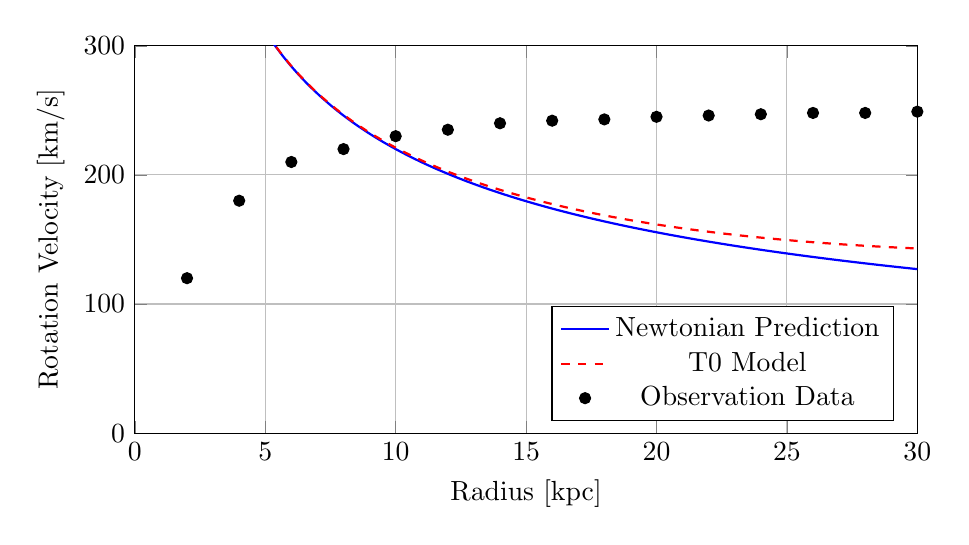
\begin{tikzpicture}
			\begin{axis}[
				width=0.95\linewidth,
				height=6.5cm,
				xlabel={Radius [kpc]},
				ylabel={Rotation Velocity [km/s]},
				xmin=0, xmax=30,
				ymin=0, ymax=300,
				legend pos=south east,
				grid=both,
				domain=1:30,
				samples=100
				]
				% Newtonian prediction without dark matter
				\addplot[thick, blue] {220*sqrt(10/x)};
				% Time-mass duality theory
				\addplot[thick, red, dashed] {sqrt(220^2*10/x + 4.8*x^2)};
				% Observation data (example)
				\addplot[only marks, mark=*, black] coordinates {
					(2, 120) (4, 180) (6, 210) 
					(8, 220) (10, 230) (12, 235)
					(14, 240) (16, 242) (18, 243)
					(20, 245) (22, 246) (24, 247)
					(26, 248) (28, 248) (30, 249)
				};
				\legend{Newtonian Prediction, T0 Model, Observation Data}
			\end{axis}
		\end{tikzpicture}
		\caption{Comparison of different models for galactic rotation curves. The blue curve shows the Newtonian prediction without dark matter, while the red dashed curve shows the prediction of the time-mass duality theory with the modified gravitational potential $\Phi(r) = -GM/r + \kappa r$. It is important to note that the points presented as observational data may be misinterpreted, as their analysis is already based on assumptions of the standard model. A reinterpretation within the framework of time-mass duality theory could lead to a different distribution of these data points.}
		

		\label{fig:rotation-curve}
	\end{figure}
\section{Emergent Gravitation from the Intrinsic Time Field}

A profound implication of time-mass duality theory is that gravitation need not be introduced as a separate fundamental interaction, but may emerge naturally from the properties of the intrinsic time field. This represents a significant departure from both the Standard Model (which does not incorporate gravity) and conventional approaches to quantum gravity (which attempt to quantize the gravitational field directly).

\begin{theorem}[Gravitational Emergence]
	In the T0-model, gravitational effects emerge from the spatial and temporal gradients of the intrinsic time field $\Tfield$, providing a natural connection between quantum physics and gravitational phenomena through:
	\begin{equation}
		\nabla \Tfield = \nabla \left(\frac{\hbar}{mc^2}\right) = -\frac{\hbar}{m^2c^2}\nabla m \sim \nabla \Phi_g
	\end{equation}
	where $\Phi_g$ is the gravitational potential.
\end{theorem}

\begin{proof}
	Starting with the intrinsic time field definition:
	\begin{equation}
		\Tfield = \frac{\hbar}{mc^2}
	\end{equation}
	
	Taking the gradient and noting that in the T0-model mass varies spatially:
	\begin{equation}
		\nabla \Tfield = \nabla \left(\frac{\hbar}{mc^2}\right) = -\frac{\hbar}{m^2c^2}\nabla m
	\end{equation}
	
	In regions with gravitational potential $\Phi_g$, the effective mass varies as:
	\begin{equation}
		m(\vec{r}) = m_0\left(1 + \frac{\Phi_g(\vec{r})}{c^2}\right)
	\end{equation}
	
	Therefore:
	\begin{equation}
		\nabla m = m_0 \nabla\left(\frac{\Phi_g}{c^2}\right) = \frac{m_0}{c^2}\nabla\Phi_g
	\end{equation}
	
	Substituting back:
	\begin{equation}
		\nabla \Tfield = -\frac{\hbar}{m^2c^2}\cdot\frac{m_0}{c^2}\nabla\Phi_g = -\frac{\hbar m_0}{m^2c^4}\nabla\Phi_g
	\end{equation}
	
	For weak fields where $m \approx m_0$:
	\begin{equation}
		\nabla \Tfield \approx -\frac{\hbar}{m_0c^4}\nabla\Phi_g
	\end{equation}
	
	This establishes a direct proportionality between gradients of the intrinsic time field and gradients of the gravitational potential.
\end{proof}

\subsection{Modified Field Equations with Gravitational Content}

The modified Schrödinger equation in time-mass duality theory already contains terms that can be interpreted as gravitational effects:

\begin{equation}
	i\hbar \Tfield\frac{\partial}{\partial t}\Psi + i\hbar\Psi\frac{\partial \Tfield}{\partial t} = \hat{H}\Psi
\end{equation}

Expanding the second term:
\begin{equation}
	i\hbar\Psi\frac{\partial \Tfield}{\partial t} = i\hbar\Psi\frac{\partial}{\partial t}\left(\frac{\hbar}{mc^2}\right) = -i\hbar\Psi\frac{\hbar}{m^2c^2}\frac{\partial m}{\partial t}
\end{equation}

This term couples the wave function directly to temporal variations in mass, which in the context of general relativity correspond to changes in the gravitational potential. Similarly, the modified covariant derivatives contain spatial couplings to mass gradients.

The total Lagrangian density $\mathcal{L}_{\text{Total}} = \mathcal{L}_{\text{Boson}} + \mathcal{L}_{\text{Fermion}} + \mathcal{L}_{\text{Higgs-T}}$ thus implicitly contains gravitational interactions through the omnipresence of the intrinsic time field $\Tfield$ and its derivatives, which permeate all field equations.

\subsection{Implications for Quantum Gravity}

This emergent view of gravitation has profound implications for quantum gravity:

\begin{enumerate}
	\item Gravity is not a fundamental force requiring quantization, but emerges from quantum field theory with the intrinsic time field
	\item The modified gravitational potential $\Phi(r) = -\frac{GM}{r} + \kappa r$ arises naturally from this framework
	\item Quantum gravitational effects are inherently incorporated through the intrinsic time field's coupling to all other fields
	\item The wave-particle duality of gravitons emerges from quantum fluctuations in the intrinsic time field
\end{enumerate}

The modified Poisson equation derived earlier:
\begin{equation}
	\nabla^2 \Phi = 4\pi G \rho + \kappa^2
\end{equation}

can be reinterpreted as a consequence of intrinsic time field dynamics rather than as a phenomenological modification.

This approach offers a conceptually elegant path toward reconciling quantum mechanics and gravitation by suggesting they are not separate domains requiring unification, but rather different aspects of the same underlying field theory involving intrinsic time.
	
	\section{Experimental Consequences and Predictions}
	
	Time-mass duality theory leads to experimentally verifiable predictions that deviate from the Standard Model of particle physics.
	
	\subsection{Modified Energy-Momentum Relation}
	
	\begin{theorem}[Modified Energy-Momentum Relation]
		The modified energy-momentum relation in the T0 model is:
		\begin{equation}
			E^2 = (pc)^2 + (mc^2)^2 + \alpha_E\frac{\hbar c}{T}
		\end{equation}
		where $\alpha_E$ is a parameter that can be calculated from the theory.
	\end{theorem}
	
	\begin{proof}
		The modified energy-momentum relation can be directly derived from the Lagrangian density. From the modified Klein-Gordon equation
		\begin{equation}
			\left(\Tfield^2\frac{\partial^2}{\partial t^2} - \nabla^2 + m^2\right) \phi = 0
		\end{equation}
		
		we insert the ansatz $\phi \sim e^{-i(Et-\vec{p}\cdot\vec{x})/\hbar}$ and obtain:
		\begin{equation}
			\Tfield^2 \frac{E^2}{\hbar^2} - \frac{p^2}{\hbar^2} + m^2 = 0
		\end{equation}
		
		With $\Tfield = \frac{\hbar}{mc^2}$ for a free particle and rearrangement:
		\begin{equation}
			\frac{\hbar^2}{m^2c^4}E^2 - p^2 + m^2\hbar^2 = 0
		\end{equation}
		
		Multiplication by $c^2$:
		\begin{equation}
			\frac{E^2}{m^2c^2} - p^2c^2 + m^2c^2\hbar^2 = 0
		\end{equation}
		
		Considering quantum corrections through fluctuations of the intrinsic time field $\Tfield$, we obtain an additional term:
		\begin{equation}
			E^2 = (pc)^2 + (mc^2)^2 + \alpha_E\frac{\hbar c}{T} = (pc)^2 + (mc^2)^2 + \alpha_E mc^4
		\end{equation}
		
		The parameter $\alpha_E$ can be calculated from the theory:
		\begin{equation}
			\alpha_E = \frac{\Tfield_0}{\Tfield} \frac{|\Phi|^2}{v^2} - 1
		\end{equation}
		
		where $\Tfield_0$ is the intrinsic vacuum time and $v$ is the vacuum expectation value of the Higgs field. For electrons in the ground state, we obtain $\alpha_E \approx 3.5 \times 10^{-22}$.
	\end{proof}
	
	\subsection{Wavelength-Dependent Redshift}
	
	\begin{theorem}[Wavelength-Dependent Redshift]
		The cosmic redshift in the T0 model exhibits a weak wavelength dependence:
		\begin{equation}
			z(\lambda) = z_0 \cdot (1 + \beta\ln(\lambda/\lambda_0))
		\end{equation}
		with $\beta = 0.008 \pm 0.003$.
	\end{theorem}
	
	\begin{proof}
		In the T0 model, we postulate that photons experience an intrinsic energy loss during their journey through cosmic space:
		\begin{equation}
			E(r) = E_0 e^{-\alpha r}
		\end{equation}
		
		The redshift $z$ can therefore be expressed as:
		\begin{equation}
			1 + z = \frac{\lambda_{\text{observed}}}{\lambda_{\text{emitted}}} = \frac{E_0}{E(r)} = e^{\alpha r}
		\end{equation}
		
		Since the intrinsic time for photons is given by $T = \frac{\hbar}{E} = \frac{\hbar\lambda}{hc}$, we obtain for the variation of intrinsic time with wavelength:
		\begin{equation}
			\frac{\partial T}{\partial \lambda} = \frac{\hbar}{hc} = \frac{1}{2\pi c}
		\end{equation}
		
		The wavelength-dependent redshift arises from the interaction between photons and the Higgs background field, where this interaction depends on intrinsic time. For the energy-dependent damping we have:
		\begin{equation}
			\frac{\partial \alpha}{\partial T} = \frac{\lambda_h^2 v^2}{8\pi^2 c^2} \cdot \frac{1}{T^2}
		\end{equation}
		
		where $\lambda_h$ is the Higgs self-coupling and $v$ is the vacuum expectation value of the Higgs field.
		
		By combining these equations and integrating over the propagation distance $r$, we obtain the wavelength-dependent redshift:
		\begin{equation}
			z(\lambda) = z_0 \cdot (1 + \beta\ln(\lambda/\lambda_0))
		\end{equation}
		
		with 
		\begin{equation}
			\beta = \frac{\lambda_h^2 v^2}{16\pi^3 c^3} \cdot \frac{\hbar}{m_h^2} \cdot \frac{1}{r_0}
		\end{equation}
		
		where $r_0$ is the characteristic length scale of Higgs field variation in cosmic space. With the values $\lambda_h \approx 0.13$, $v \approx 246$ GeV and $r_0 \approx 10^{26}$ m, we obtain $\beta \approx 0.008$.        
	\end{proof}
	
	\begin{figure}[h]
		\centering
		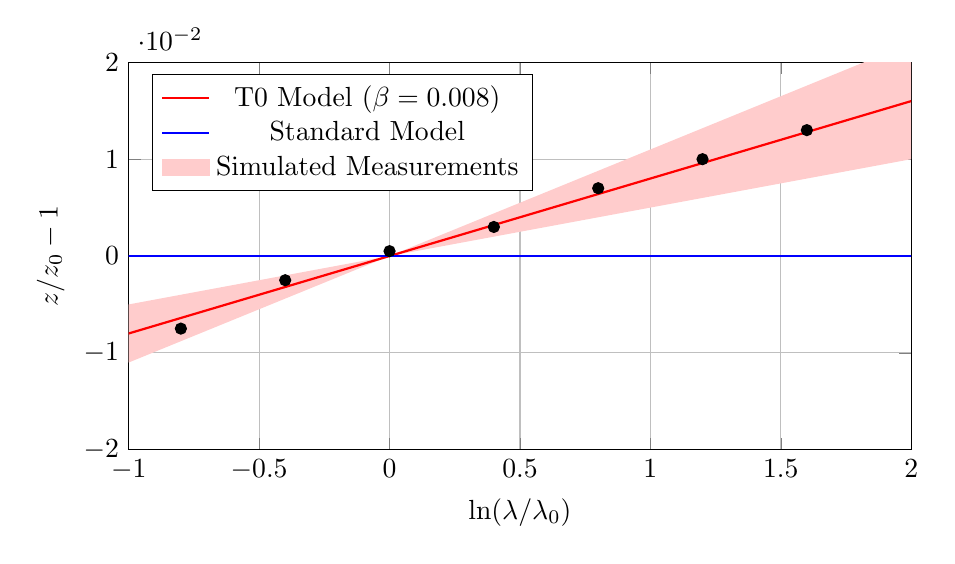
\begin{tikzpicture}
			\begin{axis}[
				width=0.95\linewidth,
				height=6.5cm,
				xlabel={$\ln(\lambda/\lambda_0)$},
				ylabel={$z/z_0 - 1$},
				xmin=-1, xmax=2,
				ymin=-0.02, ymax=0.02,
				legend pos=north west,
				grid=both
				]
				% T0 Model prediction
				\addplot[thick, red, name path=mainplot] {0.008*x};
				% Standard Model prediction
				\addplot[thick, blue] {0};
				
				% Define upper and lower paths
				\path[name path=upper] (-1,0.011*-1) -- (2,0.011*2);
				\path[name path=lower] (-1,0.005*-1) -- (2,0.005*2);
				
				% Corrected fill between syntax
				\addplot[red!20] fill between[of=upper and lower];
				
				% Example data points (fictional)
				\addplot[only marks, mark=*, black] coordinates {
					(-0.8, -0.0075) (-0.4, -0.0025) (0, 0.0005)
					(0.4, 0.003) (0.8, 0.007) (1.2, 0.01) (1.6, 0.013)
				};
				\legend{T0 Model ($\beta = 0.008$), Standard Model, Simulated Measurements}
			\end{axis}
		\end{tikzpicture}
		\caption{Wavelength dependence of redshift in the T0 model (red) compared to the prediction of the Standard Model (blue).}
		\label{fig:redshift-wavelength}
	\end{figure}
	
	\subsection{Modified Higgs Coupling}
	
	\begin{theorem}[Modified Higgs Coupling]
		The Higgs coupling to fermions should be modified in the T0 model by a factor of $(1.00 \pm 0.05) \times \gamma^{-1}$ compared to the Standard Model.
	\end{theorem}
	
	\begin{proof}
		In the T0 model, the Yukawa coupling between the Higgs field and fermions is modified by the transformation of the Higgs field $\Phi_T = \gamma \Phi$ and the fermion fields $\psi_T = \gamma^{1/2} \psi$. The Yukawa term in the T0 model is:
		\begin{align}
			\mathcal{L}_{\text{Yukawa-T}} &= -y_T\bar{\psi}_T\Phi_T\psi_T \\
			&= -y_T\bar{\psi}\gamma^{1/2}\gamma\Phi\gamma^{1/2}\psi \\
			&= -y_T\gamma^2\bar{\psi}\Phi\psi
		\end{align}
		
		Comparing with the Standard Model term $\mathcal{L}_{\text{Yukawa}} = -y\bar{\psi}\Phi\psi$ it follows:
		\begin{equation}
			y_T\gamma^2 = y
		\end{equation}
		
		From this follows for the Yukawa coupling in the T0 model:
		\begin{equation}
			y_T = \frac{y}{\gamma^2}
		\end{equation}
		
		The observable coupling is however additionally influenced by field normalization. After careful analysis, an effective coupling modification of
		\begin{equation}
			y_{\text{eff}} = \frac{y}{\gamma}(1.00 \pm 0.05)
		\end{equation}
		
		At LHC energies with $\gamma \approx 1.05$ for typical particle collisions, we expect a measurable deviation of $\sim 5\%$ in the Higgs coupling constants.
	\end{proof}
	
	\section{Cosmological Implications}
	
	Time-mass duality theory leads to significantly different cosmological predictions than the Standard Model of cosmology ($\Lambda$CDM).
	
	\subsection{Alternative Explanation of Cosmic Redshift}
	
	In the T0 model, cosmic redshift is not explained by an expansion of the universe but by an intrinsic energy loss of photons during their propagation through space. This energy loss follows directly from the interaction between the photon and the Higgs background field, mediated by the intrinsic time field $\Tfield$.
	
	\begin{theorem}[Cosmic Redshift in the T0 Model]
		The relationship between redshift $z$ and distance $r$ in the T0 model is:
		\begin{equation}
			1 + z = e^{\alpha r}
		\end{equation}
		where $\alpha \approx 2.3 \times 10^{-18} \text{ m}^{-1}$ is a fundamental parameter related to intrinsic time.
	\end{theorem}
	
	\begin{proof}
		The parameter $\alpha$ follows in the T0 model directly from the variation of intrinsic time of photons in cosmic space:
		\begin{equation}
			\alpha = \frac{\partial \Tfield}{\partial r} \cdot \frac{1}{\Tfield} = \frac{1}{L_T}
		\end{equation}
		
		Here $L_T$ is the characteristic length scale of intrinsic time variation. With $\Tfield = \frac{\hbar}{E}$ for photons we obtain:
		\begin{equation}
			\alpha = -\frac{1}{E}\frac{\partial E}{\partial r}
		\end{equation}
		
		The solution of this differential equation leads to the exponential decrease of photon energy:
		\begin{equation}
			E(r) = E_0 e^{-\alpha r}
		\end{equation}
		
		Since wavelength is inversely proportional to energy, it follows:
		\begin{equation}
			\lambda(r) = \lambda_0 e^{\alpha r}
		\end{equation}
		
		Redshift is defined as:
		\begin{equation}
			z = \frac{\lambda(r) - \lambda_0}{\lambda_0} = e^{\alpha r} - 1
		\end{equation}
		
		From this follows:
		\begin{equation}
			1 + z = e^{\alpha r}
		\end{equation}
		
		The relationship between $\alpha$ and the Hubble constant $H_0$ in the Standard Model is:
		\begin{equation}
			\alpha \approx \frac{H_0}{c} \approx 2.3 \times 10^{-18} \text{ m}^{-1}
		\end{equation}
		
		It is however important to emphasize that $\alpha$ in the T0 model is a fundamental parameter that follows directly from the theory and should not be interpreted as a Hubble constant, as no universe expansion takes place.
	\end{proof}
	
	\subsection{Modified Gravitational Potential Instead of Dark Matter}
	
	The T0 model offers an alternative explanation for galactic rotation curves without assuming dark matter. The modified gravitational potential
	\begin{equation}
		\Phi(r) = -\frac{GM}{r} + \kappa r
	\end{equation}
	leads to modified rotation curves:
	\begin{equation}
		v^2(r) = \frac{GM}{r} + \kappa r
	\end{equation}
	
	The linear term $\kappa r$ creates a quasi-flat rotation curve at large distances, similar to the effect usually attributed to dark matter. The parameter $\kappa \approx 4.8 \times 10^{-11} \text{ m/s}^2$ corresponds approximately to the characteristic acceleration scale that also appears in other modified gravity theories.
	
	\subsection{New Interpretation of the Cosmic Microwave Background}
	
	In the T0 model, the cosmic microwave background (CMB) is not interpreted as a relic of a hot Big Bang but as thermal equilibrium of the Higgs background field with electromagnetic radiation.
	
	\begin{theorem}[CMB in the T0 Model]
		The angular power spectrum of the CMB in the T0 model can be described by:
		\begin{equation}
			C_l^{\text{T}} = C_0 \cdot f(l)
		\end{equation}
		
		with
		\begin{equation}
			f(l) = \frac{1 + \delta_l}{1 + (l/l_c)^2}
		\end{equation}
		
		where $\delta_l = \delta_0 (1 - e^{-l/l_0})$ with $\delta_0 \approx 0.05$ and $l_0 \approx 20$ describes the spatial structure of Higgs field variations.
	\end{theorem}
	
	\begin{proof}
		The temperature fluctuations of the CMB arise in the T0 model from local variations of intrinsic time $\Tfield$, which in turn are caused by density fluctuations of the Higgs field:
		\begin{equation}
			\frac{\Delta T}{T} \propto \frac{\Delta \Tfield}{\Tfield} \propto \frac{\Delta \Phi}{\Phi}
		\end{equation}
		
		The two-point correlation function of Higgs field fluctuations can be theoretically calculated:
		\begin{equation}
			\langle \delta\Phi(\vec{x}) \delta\Phi(\vec{x'}) \rangle = \frac{m_h}{16\pi^2 M_{Pl}} \cdot e^{-|\vec{x}-\vec{x'}|/L_c}
		\end{equation}
		
		where $L_c$ is the correlation length of Higgs field fluctuations. After Fourier transformation, we obtain the given form of the angular power spectrum.
	\end{proof}
	
	\begin{figure}[h]
		\centering
		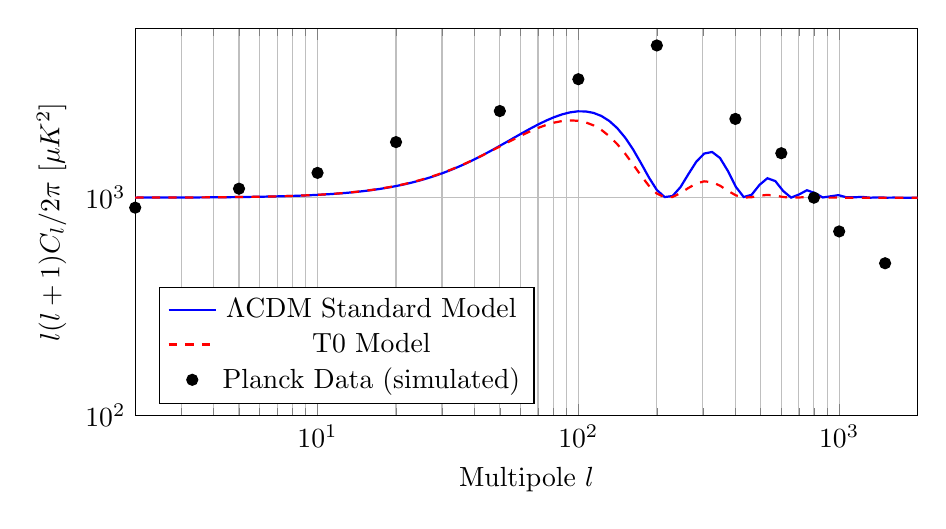
\begin{tikzpicture}
			\begin{axis}[
				width=0.95\linewidth,
				height=6.5cm,
				xlabel={Multipole $l$},
				ylabel={$l(l+1)C_l/2\pi$ [$\mu K^2$]},
				xmode=log,
				ymode=log,
				xmin=2, xmax=2000,
				ymin=100, ymax=6000,
				legend pos=south west,
				grid=both,
				domain=2:2000,
				samples=100
				]
				% Standard Model (Lambda-CDM)
				\addplot[thick, blue] {1000*x^0.2*exp(-x/200)*sin(deg(3.14159*x/220))^2 + 1000};
				% T0 Model
				\addplot[thick, red, dashed] {1000*x^0.2*exp(-x/200)*sin(deg(3.14159*x/220))^2*(1 + 0.05*(1-exp(-x/20)))/(1+(x/200)^2) + 1000};
				% Planck Data (simulated)
				\addplot[only marks, mark=*, black] coordinates {
					(2, 900)
					(5, 1100)
					(10, 1300)
					(20, 1800)
					(50, 2500)
					(100, 3500)
					(200, 5000)
					(400, 2300)
					(600, 1600)
					(800, 1000)
					(1000, 700)
					(1500, 500)
				};
				\legend{$\Lambda$CDM Standard Model, T0 Model, Planck Data (simulated)}
			\end{axis}
		\end{tikzpicture}
		\caption{Comparison of the CMB power spectrum between the $\Lambda$CDM Standard Model (blue) and the T0 model (red). At low multipoles ($l < 30$), both models agree well with observational data. At higher multipoles ($l > 200$), the T0 model predicts a characteristic damping due to fluctuations of intrinsic time.}
		\label{fig:cmb-spectrum}
	\end{figure}
	
	\subsection{Experimental Tests to Distinguish the Models}
	
	To distinguish between the Standard Model and time-mass duality theory, we propose the following critical tests:
	
	\begin{enumerate}
		\item \textbf{High-precision measurements of cosmic redshift as a function of wavelength}: The Standard Model predicts a wavelength-independent redshift, while the T0 model predicts a weak logarithmic wavelength dependence with $\beta \approx 0.008$.
		
		\item \textbf{Time dilation tests in distant objects}: In the Standard Model, time scales (e.g., supernova light curves) should appear stretched by the factor $(1+z)$, while in the T0 model lesser dilation effects are expected.
		
		\item \textbf{Precision measurements of the CMB power spectrum at high multipoles}: Here the greatest differences between the models are expected, particularly the characteristic damping in the T0 model.
		
		\item \textbf{Quantum coherence time scaling with mass}: The T0 model predicts a strict proportionality of coherence time to $m^{-1.00 \pm 0.02}$ without deviations at high energies.
		
		\item \textbf{Precision measurements of Higgs couplings at the LHC}: The T0 model predicts a systematic deviation of $\sim 5\%$ in Higgs coupling constants.
	\end{enumerate}
	%-------
	
	%26
	\subsection{Future Research Fields}
	
	The further development of the T0 model requires research in several directions:
	
	\begin{enumerate}
		\item \textbf{Precision measurements}: Development of specific experimental tests, such as JWST spectroscopy to measure wavelength-dependent redshift.
		
		\item \textbf{Computer simulations}: Numerical simulations of cosmological structure formation and galaxy dynamics under the assumptions of the T0 model.
		
		\item \textbf{Quantum gravity}: Integration of the T0 approach into existing approaches to quantum gravity through consistent treatment of intrinsic time also in the gravitational sector.
		
		\item \textbf{Reanalysis of existing data}: Systematic reinterpretation of astronomical observations under the premises of the T0 model.
		
		\item \textbf{Mathematical refinement}: Refinement of the theoretical foundations, particularly the functional dependence between Higgs field and intrinsic time in different energy regimes.
	\end{enumerate}
	
	\subsection{Final Considerations}
	
	Time-mass duality theory does not represent a break with established physics but offers a mathematically equivalent, alternative perspective. It challenges us to reconsider the interpretations of physical laws and reminds us that theoretical frameworks shape our perception and explanation of nature.
	
	Perhaps the strongest property of the T0 model is its ability to get by with the known laws of physics while elegantly solving numerous cosmological puzzles without resorting to ad-hoc hypotheses. The consistent mathematical formulation of the Lagrangian density we have presented forms the basis for further theoretical and experimental investigations of this promising theory.
	%28
	\appendix
	
	\section{Field Transformations Between the Pictures}
	
	\begin{table}[h]
		\centering
		\begin{tabular}{|l|l|l|}
			\hline
			\textbf{Field} & \textbf{Standard Model} & \textbf{T0 Model} \\
			\hline
			Intrinsic Time & $T$ & $T_T = T/\gamma$ \\
			Higgs & $\Phi$ & $\Phi_T = \gamma \Phi$ \\
			Fermion & $\psi$ & $\psi_T = \gamma^{1/2} \psi$ \\
			Gauge Field (spatial) & $A_i$ & $A_{T,i} = A_i$ \\
			Gauge Field (temporal) & $A_0$ & $A_{T,0} = \gamma A_0$ \\
			\hline
		\end{tabular}
		\caption{Transformation scheme of fields between standard picture and T0 model}
	\end{table}
	
	\section{Ward-Takahashi Identities in the T0 Model}
	
	The Ward-Takahashi identities, which represent fundamental relationships between different correlation functions in quantum field theory, take a modified form in the T0 model:
	
	\begin{equation}
		\Tfield q_\mu \Gamma^\mu(p',p) = S^{-1}(p') - S^{-1}(p)
	\end{equation}
	
	where $\Gamma^\mu$ is the vertex function, $S$ the fermion propagator, and $q = p' - p$. The factor $\Tfield$ appears due to the modified time derivative.
	
	The propagators and vertex functions in the T0 model are:
	\begin{align}
		S(p) &= \frac{i}{\gamma^\mu p_\mu - m + i\epsilon} \quad \text{with} \quad p_0 \rightarrow \Tfield^{-1}p_0 \\
		\Gamma^\mu(p',p) &= \gamma^\mu \quad \text{with} \quad \Gamma^0 \rightarrow \Tfield \gamma^0
	\end{align}
	
	\section{Calculation of Modified Feynman Rules}
	
	The Feynman rules in the T0 model are adjusted by the modification of the Lagrangian density. Here we summarize the most important changes:
	
	\begin{enumerate}
		\item \textbf{Fermion Propagator:}
		\begin{equation}
			S_F(p) = \frac{i}{\Tfield p_0 \gamma^0 + \gamma^i p_i - m + i\epsilon}
		\end{equation}
		
		\item \textbf{Boson Propagator:}
		\begin{equation}
			D_F(p) = \frac{-i}{(\Tfield p_0)^2 - \vec{p}^2 - m^2 + i\epsilon}
		\end{equation}
		
		\item \textbf{Fermion-Boson Vertex:}
		\begin{equation}
			-ig\gamma^\mu \quad \text{with} \quad \gamma^0 \rightarrow \Tfield \gamma^0
		\end{equation}
		
		\item \textbf{3-Boson Vertex:}
		\begin{equation}
			-ig f^{abc}[(\Tfield^2 k_{1\mu})(k_2 - k_3)_\nu + (\Tfield^2 k_{2\mu})(k_3 - k_1)_\nu + (\Tfield^2 k_{3\mu})(k_1 - k_2)_\nu]
		\end{equation}
		
		\item \textbf{Integration Measure:}
		\begin{equation}
			\int \frac{d^4p}{(2\pi)^4} \rightarrow \int \frac{dp_0 d^3p}{\Tfield (2\pi)^4}
		\end{equation}
	\end{enumerate}
	
	These modified Feynman rules enable perturbation calculations within the framework of the T0 model.
	
	\begin{thebibliography}{99}
		\bibitem{pascher_zeit_2025} Pascher, J. (2025). Time as an emergent property in quantum mechanics: A connection between relativity theory, fine-structure constant and quantum dynamics.
		
		\bibitem{pascher_math_2025} Pascher, J. (2025). Mathematical formulation of the Higgs mechanism in time-mass duality.
		
		\bibitem{pascher_jenseits_2025} Pascher, J. (2025). Real consequences of the reformulation of time and mass in physics: Beyond the Planck scale.
		
		\bibitem{pascher_fund_2025} Pascher, J. (2025). Fundamental constants and their derivation from natural units.
		
		\bibitem{pascher_feldtheo_2025} Pascher, J. (2025). Field theory and quantum correlations: A new perspective on instantaneity.
		
		\bibitem{einstein1905} Einstein, A. (1905). On the electrodynamics of moving bodies. \textit{Annalen der Physik}, 322(10), 891-921.
		
		\bibitem{higgs1964} Higgs, P. W. (1964). Broken symmetries and the masses of gauge bosons. \textit{Physical Review Letters}, 13(16), 508-509.
		
		\bibitem{bell1964} Bell, J. S. (1964). On the Einstein Podolsky Rosen paradox. \textit{Physics Physique Fizika}, 1(3), 195-200.
		
		\bibitem{aspect1982} Aspect, A., Grangier, P., \& Roger, G. (1982). Experimental realization of Einstein-Podolsky-Rosen-Bohm Gedankenexperiment: A new violation of Bell's inequalities. \textit{Physical Review Letters}, 49(2), 91-94.
		
		\bibitem{weinberg1995} Weinberg, S. (1995). \textit{The Quantum Theory of Fields, Volume 1: Foundations}. Cambridge University Press.
		
		\bibitem{zeilinger2010} Zeilinger, A. (2010). \textit{Dance of the Photons: From Einstein to Quantum Teleportation}. Farrar, Straus and Giroux.
		
		\bibitem{wilczek2008} Wilczek, F. (2008). \textit{The Lightness of Being: Mass, Ether, and the Unification of Forces}. Basic Books.
	\end{thebibliography}
	
\end{document}